\chapter{BI na Justiça Federal do RN}\label{cap_trabalho_academico}

% https://www.researchgate.net/publication/273861123_Why_Business_Intelligence_Significance_of_Business_Intelligence_Tools_and_Integrating_BI_Governance_with_Corporate_Governance

Na Justiça Federal do Rio Grande do Norte (JFRN) o BI é importante para entender o que está acontecendo nas diferentes Varas. O software usado é o Qlikview, que é capaz de montar gráficos e consultas a partir do banco de dados fornecido pelo Tribunal Regional Federal da $5^{a}$ região (TRF5), a distribuição dos painéis, gerados pelo Qlikview, é feita pelo portal BI do TRF5.

Nesse portal existem diferentes painéis, que atendem demandas distintas, sendo bastante usado por servidores e magistrados. Porém, o processo de desenvolvimento nesses painéis apresenta alguns gargalos, pois antes de desenvolver é necessário que hajam documentos que autorizem a criação de um novo painel, e após o desenvolvimento é necessário um outro documento autorizando a publicação desse painel. Durante o desenvolvimento também há algumas demandas que dependem do time de Tecnologia da Informação do Tribunal Regional Federal da 5ª Região (TRF5), essas demandas vão desde disponibilização de dados até renovação de licenças expiradas, essa dependência também gera alguns atrasos para o time local da JFRN. Cada desenvolvedor deve ter uma licença válida, que é paga, isso acaba aumentando o custo do desenvolvimento. 


\section{Estrutura básica do BI}

Como foi apresentado anteriormente, o BI serve para auxiliar nas tomadas de decisão, e isso é alcançado usando os dados da instituição em que estiver sendo empregado. Os dados são armazenados em \textit{Data Warehouses}(DW), que são armazéns de dados, em tradução livre, esses armazéns guardam dados históricos, então a partir deles é possível analisar o desenvolvimento de variáveis importantes e o comportamento delas de acordo com períodos que o usuário desejar, e assim identificar padrões, essa análise, que é simples, já poderia ser usada para prever possíveis mudanças na estratégia de negócios \cite{negash1}.

Após o armazém, os dados devem ser coletados e limpos, a limpeza corresponde a remoção de linhas erradas, que contenham dados errados ou faltosos, que podem atrapalhar na análise e apresentação ao gestor. Em seguida, os dados são apresentados à pessoa do negócio, que a partir das suas análises irá tomar alguma decisão que afeta a estratégia da empresa. 

Depois de carregar os dados do DW, os dados devem ser limpos, essa limpeza de dados corresponde a remoção de dados que sejam ou errados ou inexistentes, que podem causar problemas na análise de dados e na visualização que será exibida para o gestor. Imagine que num conjunto de dados sobre alturas de pessoas existe alguém com 15,5m de altura, esse dado é errado e pode causar algum distúrbio na análise, alterando a média da altura dessa amostra, por exemplo.

Após a limpeza desses dados, eles podem ser lidos pelos painéis, que geram as visualizações para os gestores, que por sua vez tomarão as decisões baseados em dados corretos.  

De forma resumida, o BI usa o DW para guardar os dados, usa um conjunto de ferramentas e técnicas para limpar e extrair os dados, essa técnica também é conhecida como \textit{Extraction, Transform, Load} (ETL), e ,finalmente, apresenta gráficos que mostram o comportamento de variáveis de interesse da instituição para o gestor, que a partir disso escolhe alguma estratégia para os rumos da empresa/órgão/setor que gerencia.

\begin{figure}[h]
	\centering
	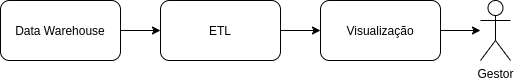
\includegraphics[scale=0.80]{./figures/cap1/resumo_bi.png}
	\caption{Resumo de um sistema BI}
\end{figure}

Isso que foi tratado acima corresponde às etapas do processamento de dados estruturados, ou seja, dados que podem ser organizados e categorizados em linhas e colunas, e que, muitas vezes, possuem relações entre si. O processo para "manusear" dados não estruturados é um pouco diferente porque eles não são tão bem organizados, e alguns passos precisam ser inseridos nesse caminho para que eles sejam apresentados e tratados da melhor forma, evitando distorções.

É possível ver que a Inteligência de Negócios é formada por várias áreas diferentes dentro da Tecnologia da Informação, a seguir estão listadas algumas:

\begin{itemize}
	\item Armazenamento na forma de \textit{Data Warehouse}
	\item Visualização de dados
	\item Mineração de dados
	\item Processamento analítico na forma de \textit{Online Analytic Processing} (OLAP)
	\item Gerenciamento do conhecimento
	\item Probabilidade
	\item Estatística
	\item Análises preditivas
	\item Detecção de anomalias
\end{itemize}

No decorrer do trabalho foram utilizados de forma mais frequente a análise de dados, a visualização e a detecção de anomalias.

\subsection{Visualização de dados}

A visualização de dados é a representação gráfica dos dados, ela engloba a produção de imagens que comunicam o comportamento e a relação dos dados analisados. Existem diferentes formas de exibição:

\begin{itemize}
	\item Gráficos de barras
	\item Histogramas
	\item Gráficos de linhas
	\item Tabelas
	\item Gráficos de dispersão
\end{itemize}

Na visualização de dados é importante transmitir o comportamento dos dados. Se um número é o dobro de outro, isso deve ser refletido na visualização, que não deve distorcer ou enganar. Ao mesmo tempo, a visualização deve ser fácil de entender. Boas representações visuais podem melhorar a mensagem da visualização. Se uma figura contém cores que não combinam, elementos visuais desequilibrados ou outras características que distraem o usuário, então será difícil de se interpretar corretamente os dados \cite{claus1}. Para que os dados sejam lidos da melhor forma, também é importante que o usuário saiba realizar interpretações, e entender sobre o que é mostrado. Por exemplo, o usuário precisa ter noções de correlação e causalidade.


\subsection{Análise de dados}

A análise de dados engloba vários processos distintos, a limpeza, transformação e modelagem dos dados fazem parte desse procedimento que pode apresentar informações relevantes onde estiver sendo aplicado. 

Para fazer uma boa análise é necessário conhecer os dados, então estudar sobre o que eles medem e sobre a realidade em que eles são aplicados, no caso da JFRN é importante entender quais são as competências das Varas, por exemplo. Para ilustrar isso um pouco melhor, imagine que numa Vara de Execução Fiscal aparecem, de acordo com os dados, muitos processos de Roubo ou Vícios de Construção, a partir disso podemos ter três hipóteses:

\begin{enumerate}
	\item Os dados estão errados
	\item A análise dos dados está errada
	\item As pessoas desconhecem a competência da Vara
\end{enumerate}

Normalmente a análise errada é responsável por alguns problemas na visualização, e cabe ao analista de dados investigar as possíveis anomalias, e descobrir se realmente houveram erros na análise ou se aconteceu algum evento diferente na Vara, por exemplo. Aqui foi tratado de um caso numa Vara, mas esse tipo de análise deve ser feito em qualquer aplicação dos dados.

É interessante notar que apesar das diversas funções que descobrem anomalias e casos extremos, ainda é importante que o analista, humano, conheça os dados e esteja sempre atualizado tanto em relação à tecnologia que será usada como também ao ramo em que estiver atuando.


\section{Custos do BI}

A Tecnologia da Informação é fundamental para o gerenciamento e manutenção correta dos negócios atualmente, ela deve ser vista como um ativo da empresa, que merece investimento em \textit{hardware}, \textit{software} e pessoal capacitado, além dos treinamentos que devem ser dados à medida que a TI expande \cite{negash1}.

\begin{itemize}
	\item \textbf{Hardware} - Os custos relacionados ao \textit{hardware} variam de acordo com a estrutura que a empresa já tiver em mãos, se um \textit{data warehouse} já existe, então a expansão precisa ser feita para um \textit{data mart}, que é uma parte dedicada aos sistemas BI. Dependendo da estrutura pode ser necessária a expansão para um sistema de redes mais robusto, que suporte o tráfego dos dados.
	
	\item \textbf{Software} - Os \textit{softwares} BI custam alto, mas também possuem muitas funcionalidades, alguns deles como o Power BI tem assinaturas a partir de \$60.000 por ano, como pode ser visto no site da \href{https://powerbi.microsoft.com/en-us/pricing/}{Microsoft}, na cotação atual isso passa de R\$300.000, então pesquisar entre os principais fornecedores do mercado é crucial para ter um preço justo e que atenda às necessidades do cliente.
	
	\item \textbf{Implementação} - Essa categoria é uma extensão da anterior porque está diretamente relacionada. Após a aquisição da ferramenta BI e do \textit{hardware} é necessário, também, realizar um treinamento do pessoal. Esse tipo de gasto também é recorrente, ou seja, sempre vai existir porque à medida que novas pessoas chegam e que o sistema expande, novos treinamentos devem ser realizados. Estima-se que esse tipo de manutenção corresponde a 15\% dos custos.
	
	\item \textbf{Pessoal} - O custo com pessoal envolve tanto quem realmente vai trabalhar com BI como envolve quem vai dar suporte às atividades de BI. Por exemplo, o time de infraestrutura deve estar preparado com as tecnologias de engenharia de dados, e manutenção do servidor que armazena os dados do BI.
	
\end{itemize}

\subsection{Exemplos de ferramentas}

Existem muitas ferramentas BI no mercado hoje, com o crescimento da área também houve a maior oferta de ferramentas que fazem painéis mais rápidos ou de forma mais simples, exigindo menos treino ou menos infraestrutura. Alguns serviços também oferecem a computação em nuvem, e "alugam" o poder computacional de acordo com o uso do cliente. Com a grande variedade de produtos também vem uma grande diferença de preços. Podemos citar, novamente, o Power BI, um dos líderes nesse tipo de atividade, custando (em 2020) \$4.995 por mês para o serviço \textit{Premium}, e esse preço pode aumentar de acordo com os serviços extra que o cliente desejar incluir no pacote.

\begin{figure}[h]
	\centering
	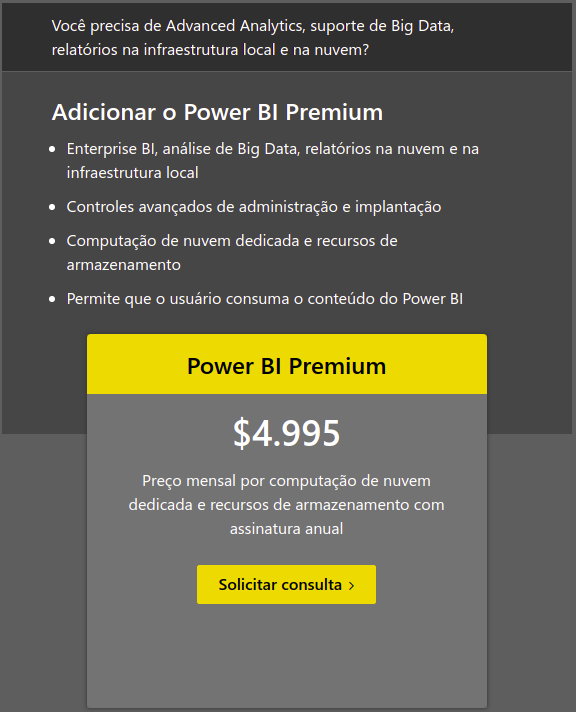
\includegraphics[scale=0.40]{./figures/cap1/powerbi.png}
	\caption{Preço do Power BI Premium \\ fonte: Microsoft}
\end{figure}


Além do Power BI podemos citar o Qlikview, que é usado na JFRN. Ele é desenvolvido pela Qlik, que ultimamente vem focando os esforços e investimentos no Qlik Sense, que oferece várias vantagens. O Qlikview foi o principal produto da Qlik durante muito tempo, a primeira versão dele data de 1994, e recebeu várias melhorias ao longo dos anos, se adequando às novas tecnologias e incorporando funções diferentes. Atualmente a Qlik tenta levar os clientes do QlikView para o Qlik Sense, que fornece painéis em plataformas móveis (\textit{smartphones} por exemplo), integração com APIs e construção de visualização simplificada, através de recursos como clique-e-arraste. Os preços variam de 40 a 70 dólares, por mês por licença.

\begin{figure}[h]
	\centering
	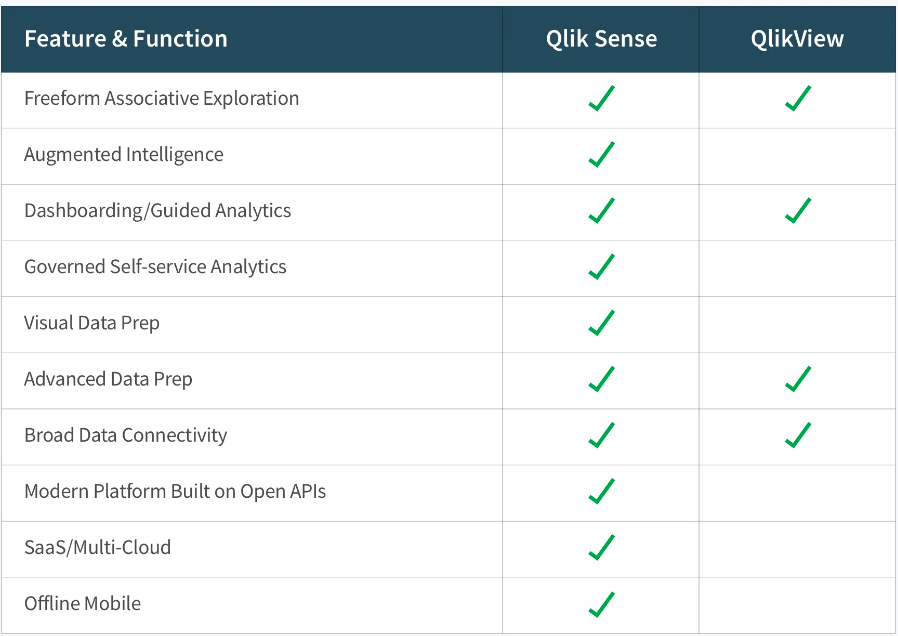
\includegraphics[scale=0.40]{./figures/cap1/qlikview.png}
	\caption{Qlikview versus Qlik Sense \\ fonte: Qlik}
\end{figure}



%https://primaconsulting.co.uk/news/2018/3/26/qlikview-vs-qliksense


